\setlength{\footskip}{8mm}

\chapter{EXPERIMENTS}


\section{Rationale}
The primary objective of these experiments is to rigorously evaluate the clinical viability, computational efficiency, and reasoning accuracy of the proposed ALIGN-VQA architecture. Traditional Medical Visual Question Answering (Med-VQA) models often falter when applied to longitudinal tasks because they are vulnerable to spatial misalignments and struggle to isolate true disease progression from harmless acquisition noise. Therefore, the experimental design is motivated by three key goals. First, the author argues that spatial misalignments and stochastic acquisition variability between historical and current scans compromise direct feature comparison. Thus, the Cross-Image Difference Attention (CIDA) module is evaluated on its ability to semantically reconstruct and align the prior-visit features to establish a reliable, misalignment-tolerant baseline. Second, rather than assuming all raw pixel-wise differences are clinically relevant, the author hypothesizes that a Learnable Residual Gating mechanism is required to actively filter out non-pathological visual noise and static anatomy, ensuring that only precise, evolution-aware features are extracted. Finally, because the vast majority of regions in a longitudinal chest X-ray remain unchanged, the author evaluates the Question-Guided Difference Tokenizer (QDT) to determine if selectively pooling a sparse subset of highly relevant tokens enables the model to perform targeted diagnostic reasoning while maintaining a highly efficient, lightweight architecture.


\section{Dataset}
To test these hypotheses, the author utilizes \cite{medical-diff-vqa}, which is a specialized derivative of the large-scale \cite{mimic-cxr}. Each sample in this dataset is structured as a longitudinal pair consisting of a historical reference radiograph and a more recent follow-up scan, stored in Digital Imaging and Communications in Medicine (DICOM) format. The x-rays images in Joint Photographic Experts Group (JPEG) format are fetched from \cite{mimic-cxr-jpg} for faster preprocessing and training. These pairs are accompanied by clinically grounded questions that specifically target temporal changes, such as the progression of pleural effusion or the placement of medical devices. The dataset comprises 164,324 pairs of main and reference chest X-ray images, yielding a total of 700,703 question-answer pairs. This high volume of data allows the model to learn the subtle semantic nuances required to distinguish between common clinical conditions like consolidation, edema, and atelectasis within a comparative context. Following standard benchmarking protocols, the dataset is strictly partitioned into training, validation, and testing sets using an 8:1:1 ratio. The Figure shows the distribution of seven distinct clinical categories

\subsection{Pathological Distribution}
Figure \ref{fig:medical_findings} illustrates the prevalence of medical findings across the dataset. The distribution exhibits a heavy long-tail characteristic typical of medical datasets. "No Finding" and "Support Devices" are the most prevalent positive labels, reflecting the high frequency of routine exams and Intensive Care Unit (ICU) patient monitoring in \cite{mimic-cxr}. Among true pathological findings, "Pleural Effusion," "Lung Opacity," and "Atelectasis" occur most frequently. Conversely, critical but less frequent findings like "Fracture" and "Pleural Other" appear significantly less often. This class imbalance highlights the necessity for robust representation learning, particularly the Counterfactual Regularizer in the ALIGN-VQA architecture, to prevent the model from defaulting to high-frequency predictions.

\begin{figure}[htbp]
	\centering
	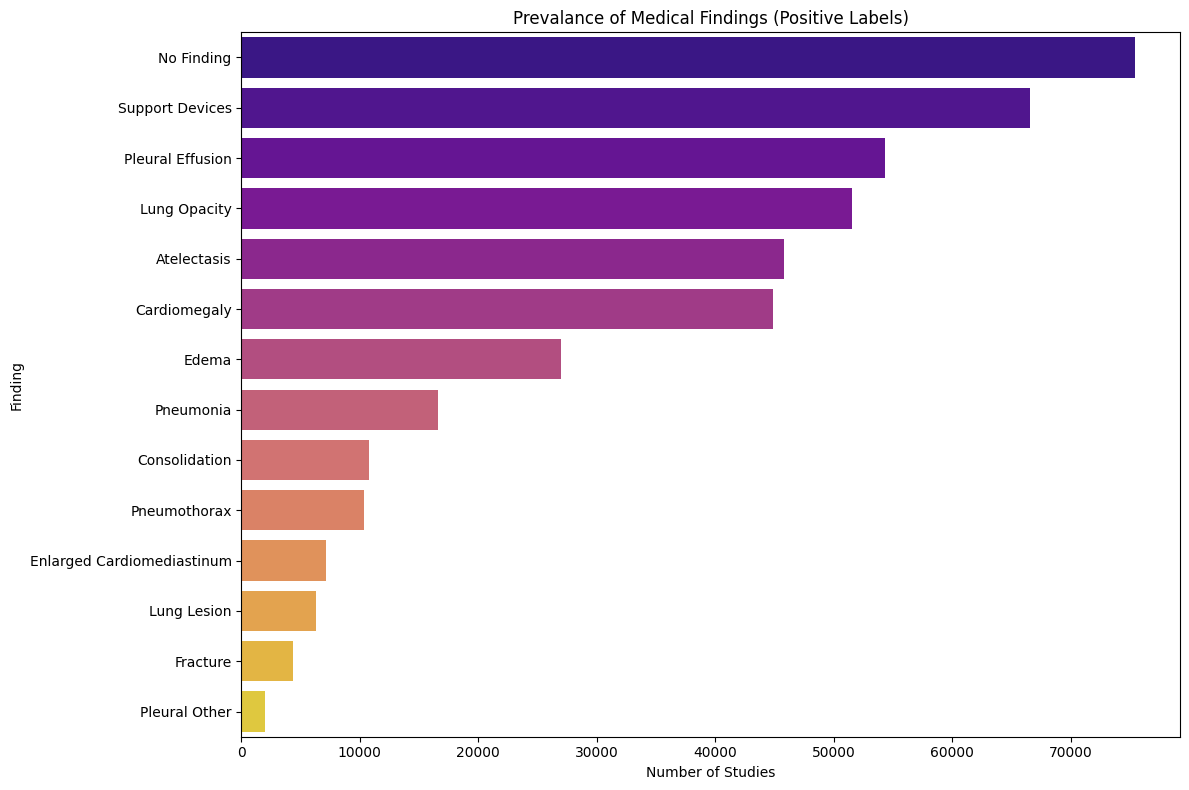
\includegraphics[width=0.9\textwidth]{figures/medical_findings.png}
	\caption{Prevalance of Medical Findings}
	\label{fig:medical_findings}
\end{figure}

\subsection{Question Type Distribution}
The questions are categorized into seven distinct clinical types, as shown in Figure \ref{fig:question_types}. The distribution is relatively balanced among the top categories, ensuring a diverse evaluation of the model's capabilities. The "Difference" category is the most frequent accounting for approximately 23 percent of the dataset, followed closely by "Presence", 22 percent and "Abnormality" 21 percent. The remaining categories—Location, Level, View, and Type—make up the rest of the dataset. While the ALIGN-VQA model is trained and evaluated across all seven categories, the primary focus of these experiments remains the "Difference" subset, as it explicitly tests the model's ability to reason about longitudinal spatial and pathological changes between the reference and current scans.

\begin{figure}[htbp]
	\centering
	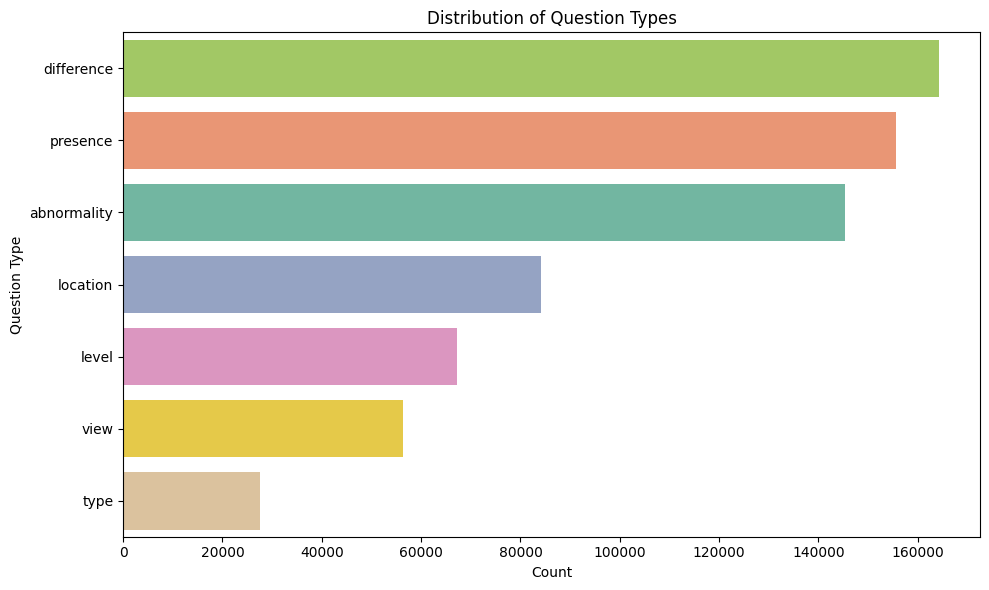
\includegraphics[width=0.9\textwidth]{figures/question_types.png}
	\caption{Distribution of Question Types}
	\label{fig:question_types}
\end{figure}

\subsection{Linguistic Distribution}
Figure \ref{fig:question_lengths} visualizes the distribution of question and answer lengths in characters. The question lengths exhibit a highly structured, multi-modal distribution with distinct peaks around 30, 42, and 50 characters. This rigid structure suggests that the questions were generated using a programmatic or templated approach based on the original radiology reports, rather than free-form human querying. The answer lengths are heavily skewed, with the vast majority of answers being extremely concise, under 25 characters, corresponding to binary "yes/no" answers or short categorical responses. A smaller, secondary distribution of longer answers, 50 to 150 characters, corresponds to the complex, descriptive answers required for the "Difference" and "Abnormality" question types.

\begin{figure}[htbp]
	\centering
	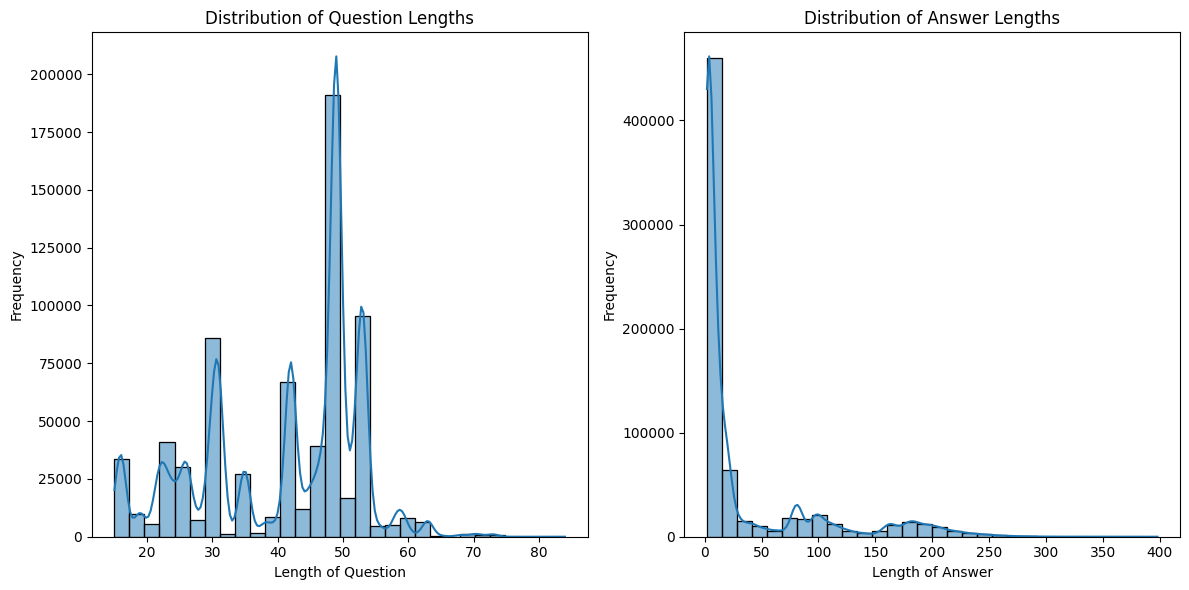
\includegraphics[width=0.9\textwidth]{figures/question_lengths.png}
	\caption{Distribution of Question Lengths}
	\label{fig:question_lengths}
\end{figure}


\section{Experiment Setting}

\subsection{Preprocessing}
To ensure standardized inputs for the vision-language pipeline, rigorous preprocessing protocols were applied to both the imaging and textual data. The resizing pipeline is engineered to maximize computational efficiency while preserving critical clinical details. Both historical and current chest X-rays were resized to $224 \times 224$ pixels to match the input dimensions expected by the tiny varient of \cite{swin}. Standard normalization was applied using \cite{cxr-clip} pretraining statistics to ensure stable feature extraction. Clinical questions were tokenized using \cite{bio-clinical-bert}, with sequences padded and truncated to a maximum length of 48 tokens. To prevent index-out-of-bounds errors and size mismatches during evaluation, a common issue when dataset splits yield varying unique word counts, the inference scripts were programmed to dynamically extract the exact expected vocabulary size directly from the saved model checkpoints prior to initializing the classification head.

\subsection{Models and Techniques}
To benchmark the proposed ALIGN-VQA architecture, its performance is compared against several state-of-the-art models that encompass both general domain change-captioning and specialized medical Diff-VQA. Among the specialized medical models, the author evaluates \cite{ekaid}, a foundational Diff-VQA framework that relies on pre-extracted bounding boxes and an anatomical knowledge graph to model changes. The author also compares the method with \cite{plural}, a computationally intensive transformer framework that utilizes massive external pretraining on natural images and radiology reports to process dense, unpruned feature concatenations. Additionally, the author benchmarks against \cite{regiomix}, a Retrieval-Augmented Generation (RAG) approach that generates pseudo-difference descriptions by mixing and matching retrieved regions from an external database. Furthermore, the author includes two recent generative medical VQA architectures including \cite{real}, which employs a dedicated residual encoder and residual feature alignment to capture image disparities, and \cite{encoder-decoder}, which utilizes \cite{swin} coupled with image differentiation embeddings to distinguish temporal scans prior to decoding.

Against these baselines, the author evaluate the proposed ALIGN-VQA, an alignment-guided residual modeling architecture featuring CIDA, a learnable gating mechanism, and the QDT. Beyond direct comparisons, extensive ablation studies are conducted on ALIGN-VQA by systematically toggling key components. For instance, the CIDA module is disabled to force direct feature subtraction, and the QDT Top-K selection threshold is altered. This allows the author to rigorously isolate and quantify the individual contributions of these novel mechanisms to the overall diagnostic accuracy.

\subsection{Training Procedure}
The model was implemented in \cite{pytorch} and trained end-to-end to ensure full reproducibility. All training procedures were executed on NVIDIA RTX6000 to efficiently accommodate the required batch sizes and the computational overhead of the attention matrix operations. The network was optimized using the AdamW optimizer with a batch size of 128. To ensure smooth convergence, the initial learning rate was set to $5 \times 10^{-5}$ and governed by a cosine annealing scheduler.

The training process strictly adhered to a multi-stage strategy designed to incrementally build the model's reasoning capabilities. This schedule commenced with one initial epoch of self-supervised Masked Residual Modeling (MRM), followed by three warm-up epochs, and concluded with 20 epochs of end-to-end Diff-VQA fine-tuning. The compound loss function was balanced using empirically derived weights, applying a weight of 1.0 to the language generation loss, 0.1 to the MRM loss, 0.1 to the counterfactual loss, and 0.5 to the auxiliary classification loss. Finally, early stopping was implemented based on validation CIDEr scores to continually monitor generalization and prevent overfitting during the fine-tuning phase.

\subsection{Evaluation Metrics}
Because automated metrics often struggle to capture the clinical nuance of medical texts, the evaluation strategy utilizes a robust mix of strict string-matching, semantic similarity, and human validation. For automated assessment, the author reports standard Natural Language Generation (NLG) metrics, including \cite{bleu}, \cite{meteor}, and \cite{rouge}, to evaluate sequence overlap and structural fluency. The author places a heavy priority on the \cite{cider} metric, as its weighting mechanism explicitly penalizes generic answers and rewards the accurate generation of rare, clinically vital keywords, such as specific pathology names.

\begin{comment}

\section{Quantitative Results on the MIMIC-Diff-VQA Benchmark}
Table 5.1 presents the quantitative performance of the proposed ALIGN-VQA against current state-of-the-art models on the \cite{medical-diff-vqa}. The evaluated baselines include early graph-based methods, retrieval-augmented models, dense-feature frameworks, and residual-based generative models.

As the results indicate, while models like \cite{encoder-decoder} and \cite{real} achieve marginally higher scores on strict n-gram overlap metrics, the proposed model establishes a new state-of-the-art on the most clinically vital metrics: \cite{meteor} (0.480), \cite{rouge} (0.739), and \cite{cider} (2.427). This distinction is critical. \cite{bleu} uniformly weights all words, heavily rewarding the generation of common syntax templates. In contrast, \cite{cider} penalizes generic, high-frequency phrases while heavily rewarding the accurate prediction of rare, informative keywords such as specific pathology names or directional clinical terms. ALIGN-VQA’s dominant \cite{cider} score of 2.427—outperforming the highly competitive \cite{real} (2.409) and vastly exceeding dense-feature models like \cite{encoder-decoder} (2.119) and \cite{plural} (1.832)—demonstrates that the extreme, QDT successfully filters out background noise without losing crucial diagnostic indicators.

\section{Ablation Studies and Component Analysis}
To isolate the contributions of the core architectural innovations, the author conducted extensive ablation studies, the results of which are detailed in Table 5.2. We evaluated the model by systematically toggling the CIDA module, CF-Reg, and varying the Top-$k$ threshold in the QDT.

\subsection{Impact of Architectural Modules}
The baseline configuration without CIDA and CF-Reg performs poorly, yielding \cite{cider} of just 1.213. Introducing the CF-Reg alone improves the metric to 1.956, confirming its role in mitigating hallucinations. Conversely, introducing CIDA alone (Row 4) significantly boosts the metric to 2.172, providing empirical proof that explicitly resolving spatial misalignment before calculating residuals is far superior to direct feature subtraction. Combining both modules yields the optimal the score of 2.427, demonstrating that robust spatial alignment and causal, hallucination-free reasoning are highly complementary.

\subsection{Impact of Token Sparsity}
The author also investigated the effect of the token selection threshold, $k$, within the QDT module. Setting $k$ too low ($k=12$) limits the visual evidence available to the language decoder, dropping \cite{cider} to 2.258. Conversely, increasing the threshold ($k=49$) incorporates excessive visual noise and irrelevant anatomical changes, diluting the clinical signal and lowering the metric to 2.226. The empirical sweet spot of $k=16$ ensures that the model remains highly focused on the exact pathological deviations referenced by the clinical question.

\begin{table}[htbp]
	\centering
	\caption{Quantitative performance comparison of the proposed model against state-of-the-art methods on the MIMIC-Diff-VQA dataset.}
	\label{tab:main_results_old}
	\renewcommand{\arraystretch}{1.2}
	% Resizebox scales the table to perfectly fit the text width
	\resizebox{\textwidth}{!}{%
		\begin{tabular}{l ccccccc}
			\toprule
			\textbf{Model} & \textbf{BLEU-1} & \textbf{BLEU-2} & \textbf{BLEU-3} & \textbf{BLEU-4} & \textbf{METEOR} & \textbf{ROUGE-L} & \textbf{CIDEr} \\
			\midrule
			\cite{ekaid}    & 0.624 & 0.541 & 0.477 & 0.422 & 0.337 & 0.645 & 1.893 \\
			\cite{regiomix} & 0.705 & 0.633 & 0.572 & 0.517 & 0.381 & 0.651 & 1.804 \\
			\cite{plural}   & 0.704 & 0.633 & 0.575 & 0.520 & 0.381 & 0.653 & 1.832 \\
			\cite{encoder-decoder}      & 0.716 & 0.647 & 0.590 & 0.537 & 0.389 & 0.670 & 2.119 \\
			\cite{real}     & 0.710 & 0.636 & 0.580 & 0.530 & 0.395 & 0.736 & 2.409 \\
			%MENDER   & 0.635 & 0.568 & 0.518 & 0.457 & 0.354 & 0.615 & 1.684 \\
			\midrule
			\textbf{Ours} & \textbf{0.653} & \textbf{0.578} & \textbf{0.518} & \textbf{0.466} & \textbf{0.480} & \textbf{0.739} & \textbf{2.427} \\
			\bottomrule
		\end{tabular}%
	}
\end{table}

\begin{table}[htbp]
	\centering
	\caption{Ablation studies isolating the impact of the Top-$k$ selection threshold, Cross-Image Difference Attention (CIDA), and Counterfactual (CF) regularizer.}
	\label{tab:ablation_old}
	\renewcommand{\arraystretch}{1.2}
	% Resizebox scales the table to perfectly fit the text width
	\resizebox{\textwidth}{!}{%
		\begin{tabular}{c c c ccccc c c}
			\toprule
			\textbf{Top-$k$} & \textbf{CIDA} & \textbf{CF} & \textbf{BLEU-1} & \textbf{BLEU-2} & \textbf{BLEU-3} & \textbf{BLEU-4} & \textbf{METEOR} & \textbf{ROUGE-L} & \textbf{CIDEr} \\
			\midrule
			12 & $\checkmark$ & $\checkmark$ & 0.636 & 0.541 & 0.502 & 0.450 & 0.481 & 0.700 & 2.258 \\
			49 & $\checkmark$ & $\checkmark$ & 0.631 & 0.555 & 0.496 & 0.445 & 0.480 & 0.713 & 2.226 \\
			16 & $\times$     & $\times$     & 0.399 & 0.340 & 0.296 & 0.256 & 0.274 & 0.485 & 1.213 \\
			16 & $\checkmark$ & $\times$     & 0.643 & 0.565 & 0.504 & 0.453 & 0.457 & 0.660 & 2.172 \\
			16 & $\times$     & $\checkmark$ & 0.661 & 0.577 & 0.511 & 0.453 & 0.454 & 0.661 & 1.956 \\
			\midrule
			\textbf{16} & $\checkmark$ & $\checkmark$ & \textbf{0.653} & \textbf{0.578} & \textbf{0.518} & \textbf{0.466} & \textbf{0.480} & \textbf{0.739} & \textbf{2.427} \\
			\bottomrule
		\end{tabular}%
	}
\end{table}

\end{comment}